\section{Introduction}

Metaphor texts differ in how familiar, meaningful, and easy to imagine they are, as well as in how strongly they convey figurative meaning. Researchers use ratings of these properties to select materials and compare experimental conditions. Chinese metaphor datasets record such judgments as mean human ratings on defined scales \citep{huang2024cogmed,wang2022normed}. As new materials are introduced, researchers need scores on the same dimensions. This motivates multidimensional continuous scoring: given an expression and a rating dimension, predict its mean human rating within the specified interval.

\begin{figure*}[t!]
\centering
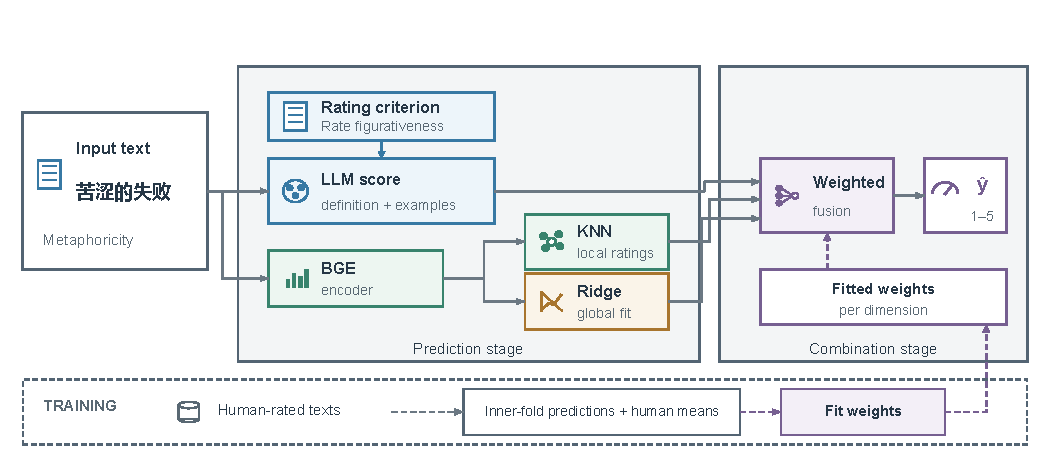
\includegraphics[width=\textwidth]{figures/fig_cems_architecture.pdf}
\caption{CEMS predicts one rating dimension for an input expression. The LLM uses the dimension criterion and rated examples; frozen BGE embeddings feed a nearest-neighbor predictor and a Ridge regressor. The combiner applies dimension-specific weights and an intercept. Dashed arrows show training: inner-fold predictions are paired with human means to fit the combiner.}
\label{fig:cems}
\end{figure*}

Automated essay scoring (AES) offers a relevant starting point. AES assigns numerical scores to texts according to assessment criteria, including separate scores for different writing traits \citep{do2024arts,eltanbouly2025trates}. Metaphor scoring shares this need to connect a judgment about text to a bounded numerical scale. Individual essay grades may be discrete, while the mean human ratings predicted here are continuous. The methodological connection is the use of explicit criteria and human-scored examples to guide numerical prediction. It allows us to draw on text-scoring methods developed in education when designing a scorer for metaphor-related properties.

In particular, rubric-based approaches make the dimensions of assessment explicit. TRATES uses trait-specific rubric questions to derive features for essay scoring \citep{eltanbouly2025trates}. AutoSCORE, developed for scoring student responses, separates the extraction of rubric-relevant components from the assignment of a score \citep{wang2026autoscore}. These methods concern educational assessment; they were not proposed for metaphor scoring. We borrow the principle of evaluating text against stated criteria, and adapt the criteria and prediction target to human judgments of metaphor texts.

This adaptation requires more than replacing an essay with a shorter expression. Essay rubrics assess aspects of student performance, whereas metaphor rating dimensions describe properties of an expression. A familiar expression need not be highly figurative, and a high score on one property does not imply a high score on another. Each predicted score must correspond to the definition of its dimension. It must also place that judgment on the scale used by human raters: a description such as ``familiar'' does not by itself specify a numerical mean. Existing human-rated expressions provide examples of how the definitions are used and where texts fall on the scale.

Our question is how to combine judgments guided by dimension definitions with the numerical information in existing human ratings. The definitions specify what to assess; rated texts show how people use the scale. We study this combination for continuous prediction across metaphor-related dimensions. We introduce CEMS, which connects an LLM's interpretation of each rating definition with predictions learned from rated examples. The LLM receives the definition, a rating question, and examples from the training set. A nearest-neighbor predictor estimates the score from semantically similar rated expressions, while an embedding regression model learns text--score relationships across the training set. Their scores are combined using weights fitted separately for each dimension, allowing the contributions of the predictors to vary with the rated property.

We evaluate CEMS on COGMED and Wang's Chinese sentence ratings. The experiments compare its numerical predictions with human means, examine item rankings, and test the contribution of each predictor. We also implement task-specific adaptations of AutoSCORE and RULERS-guided direct scoring, a rubric-based approach to general text evaluation \citep{hong2026rulers}. These comparisons examine how different scoring procedures carry over to metaphor ratings. 

Our contributions are:
\begin{itemize}[leftmargin=*,nosep]
    \item We develop an AES-inspired approach to multidimensional continuous scoring of Chinese metaphor texts, with metaphor-related rating definitions and mean human scores as the prediction target.
    \item We introduce CEMS, which combines criterion-guided LLM scores with predictions from semantically similar rated expressions and embedding regression, using dimension-specific weights learned from training data.
    \item We evaluate continuous scoring on two Chinese datasets through comparisons with individual predictors and adapted scoring frameworks, component ablations, and analyses of item ranking.
\end{itemize}


